\section{Архитектура системы планирования производства}
\indent Система планирования производства представляет из себя набор программных модулей, взаимодействующих согласно схеме (рисунок \ref{fig:archSPP}).

\begin{figure}[ht]
	\centering
	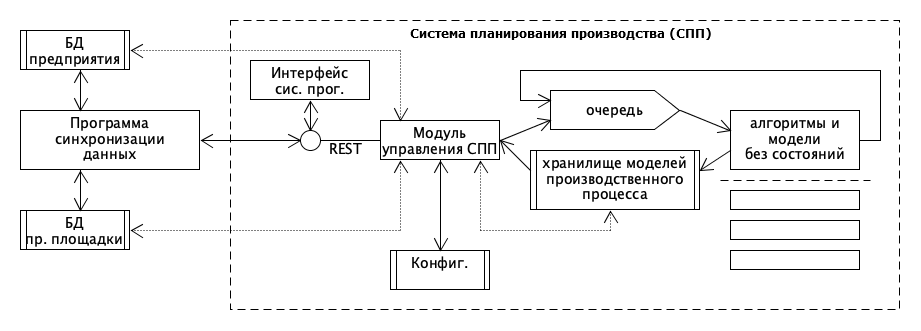
\includegraphics[width=\linewidth]{pics/archSPP.png}
	\caption{Схема системы планирования производства \cite{niorkpz}}
	\label{fig:archSPP}
\end{figure}

\indent Так как для выбора оптимального плана сотруднику требуется несколько планов, непосредственно из которых нужно будет оптимальный, система производит запуск множества параллельных расчетов, каждый из которых отличается конфигурацией смен либо количества доступных ресурсов.
За запуск и синхронизацию отвечает ``Модуль управления СПП'' (рисунок \ref{fig:archSPP}), который создает очередь расчетов на запуск.
Затем пул потоков извлекает их в порядке очереди и начинает работу ядра имитационного моделирования (``Алгоритмы и модели без состояний'', рисунок \ref{fig:archSPP}).
После окончания работы полученный результат передается обратно в модуль управления для возврата пользователю посредством RESTful API (REST~-~архитектурный стиль взаимодействия компонентов распределённого приложения в сети).
Пользователь, зная с какими параметрами запускался полученный расчет, может поменять конфигурацию и отправить его на повторное вычисление, что будет сохранено в базе данных предприятия и приведет к запуску всего цикла с начала.